% This file was created by tikzplotlib v0.9.2.
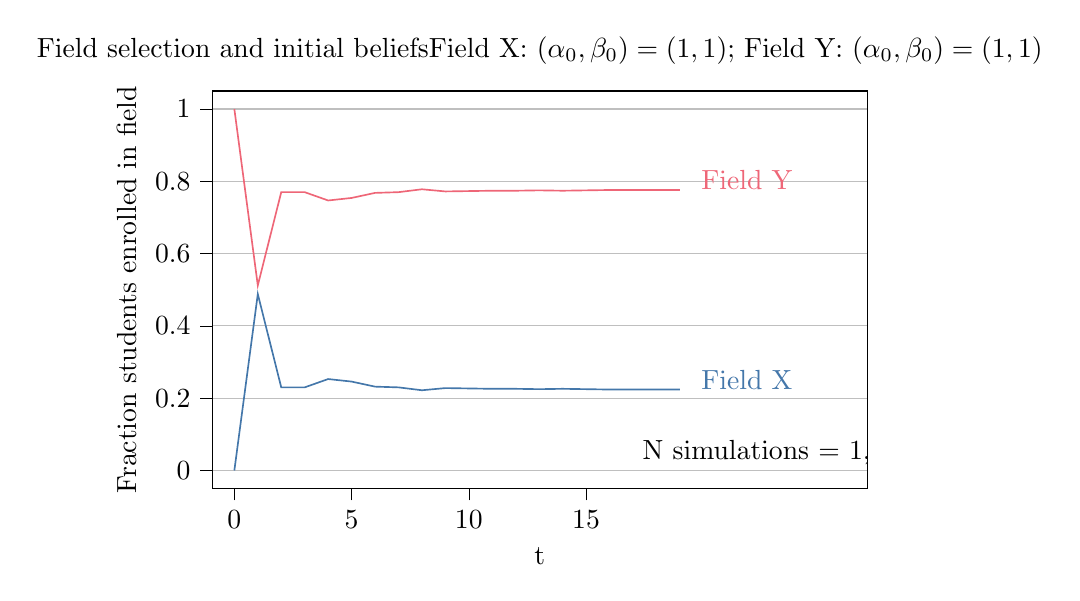
\begin{tikzpicture}

\definecolor{color0}{rgb}{0.266666666666667,0.466666666666667,0.666666666666667}
\definecolor{color1}{rgb}{0.933333333333333,0.4,0.466666666666667}

\begin{axis}[
height=6.6314113761540705cm,
tick align=outside,
tick pos=left,
title={Field selection and initial beliefs \\ Field X: \(\displaystyle (\alpha_{0}, \beta_{0}) = (1, 1)\); Field Y: \(\displaystyle (\alpha_{0}, \beta_{0}) = (1, 1)\)},
width=9.904475999999999cm,
x grid style={white!69.0196078431373!black},
xlabel={t},
xmin=-0.95, xmax=27,
xtick style={color=black},
xtick={0,5,10,15},
xticklabels={\(\displaystyle 0\),\(\displaystyle 5\),\(\displaystyle 10\),\(\displaystyle 15\)},
ylabel={Fraction students enrolled in field},
ymajorgrids,
ymin=-0.05, ymax=1.05,
ytick style={color=black},
ytick={0,0.2,0.4,0.6,0.8,1},
yticklabels={\(\displaystyle 0\),\(\displaystyle 0.2\),\(\displaystyle 0.4\),\(\displaystyle 0.6\),\(\displaystyle 0.8\),\(\displaystyle 1\)}
]
\addplot [semithick, color0]
table {%
0 0
1 0.48800003528595
2 0.230000019073486
3 0.230000019073486
4 0.253000020980835
5 0.246000051498413
6 0.23199999332428
7 0.230000019073486
8 0.222000002861023
9 0.228000044822693
11 0.22599995136261
12 0.22599995136261
13 0.225000023841858
14 0.22599995136261
16 0.223999977111816
19 0.223999977111816
};
\addplot [semithick, color1]
table {%
0 1
1 0.51200008392334
2 0.769999980926514
3 0.769999980926514
4 0.746999979019165
5 0.753999948501587
6 0.76800000667572
7 0.769999980926514
8 0.777999997138977
9 0.772000074386597
11 0.773999929428101
12 0.773999929428101
13 0.774999976158142
14 0.773999929428101
16 0.776000022888184
19 0.776000022888184
};
\draw (axis cs:19.5,0.224) node[
  anchor=base west,
  text=color0,
  rotate=0.0
]{Field X};
\draw (axis cs:19.5,0.776) node[
  anchor=base west,
  text=color1,
  rotate=0.0
]{Field Y};
\draw (axis cs:17,0.03) node[
  anchor=base west,
  text=black,
  rotate=0.0
]{N simulations = 1,000};
\end{axis}

\end{tikzpicture}
